%
% split.tex
%
\renewcommand{\thisname}{Chart::Split}
\section{\thisname}
\name{\thisname}
\file{Split.pm}
\requires{Chart::Base, GD, Carp, FileHandle}
\begin{Description}
The class \thisclass creates a lines chart where both $x$ and $y$ axes
are assumed to be numeric. Split charts are mainly intended for cases
where many data points are spread over a wide $x$ range while at the
same time the $y$ range is limited. Typical examples are weather or
seismic data. The $x$ axis will be split into several intervals of the
same length (specified with the mandatory option \attruse{interval}).
The intervals will be displayed in a stacked fashion. The start of the
top interval is set with the mandatory option \attruse{start}.
\thisclass will draw only positive $x$ coordinates. The $y$ axis will
not be labelled with the $y$ values. Rather, the axis will show only
the sequence numbers of the intervals. \thisclass is a subclass of
\class{Chart::Base}.
\end{Description}

\example

\begin{figure}[ht]
  \begin{center}
    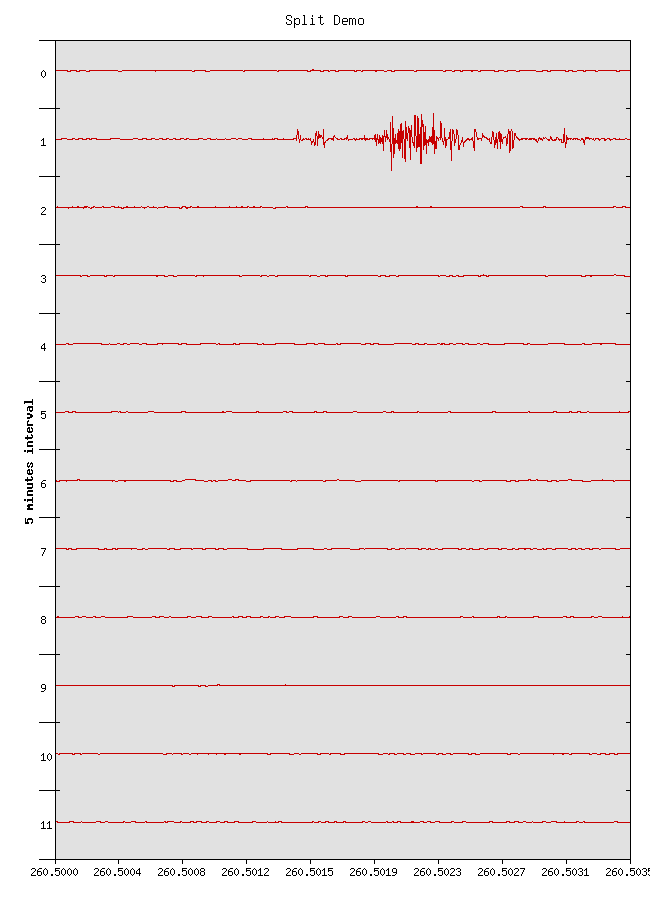
\includegraphics[width=\textwidth, height=\textwidth]{stunde.png}
  \end{center}
  \caption{Split chart}
  \label{fig:split}
\end{figure}
\begin{verbatim}
use Chart::Split;

$g = Chart::Split->new(650, 900);

# Get the data from a file and push them into arrays
open(FILE, "data.dat") or die "Can't open the data file!\n";
while (<FILE>) {
  ($x, $y) = split;
   push (@x, $x);
   push (@y, $y);
}
close(FILE);

# Add the data
$g->add_dataset(@x);
$g->add_dataset(@y);

# Set the options
$g->set('xy_plot'        => 'true');
$g->set('legend'         => 'none');
$g->set('title'          => 'Split Demo');
$g->set('interval'       => 1/288);
$g->set('interval_ticks' => 10);
$g->set('start'          => 260.5);
$g->set('brush_size'     => 1);
$g->set('precision'      => 4);
$g->set('y_label'        => '5 minutes interval');

# Give me a nice picture
$g->png("split.png");
\end{verbatim}

\constructorblurb{\thisname}

\begin{AttrDecl}{start}
Sets the start value of the first interval. If the $x$ coordinate of
the first data point is 0, \attruse{start} should also be set to 0.
\emph{Required} value for a \thisclass chart. Defaults to undef.
\end{AttrDecl}

\begin{AttrDecl}{interval}
Sets the interval of one segment to plot. \emph{Required} value for a
split chart. Defaults to undef.
\end{AttrDecl}

\begin{AttrDecl}{interval\_ticks}
Sets the number of ticks for the $x$ axis. Defaults to 5.
\end{AttrDecl}

\begin{AttrDecl}{scale}
Every $y$ value of a \thisclass chart will be multiplied by this value,
without however changing the sclaing of the $y$ axis. (This might result
in some segments being overdrawn by others.) Only useful if you want to
give prominence to the maximal amplitudes of data. Defaults to 1.
\end{AttrDecl}

\begin{AttrDecl}{sort}
Sorts the data in ascending order if set to \literal{true}. Should be set if
the input data is not sorted. Defaults to \literal{false}.
\end{AttrDecl}

\begin{AttrDecl}{y\_axes}
Tells \thisclass where to place the $y$ axis. Valid
values are \literal{left}, \literal{right} and \literal{both}. Defaults
to \literal{left}.
\end{AttrDecl}
